
\documentclass[11pt,a4paper]{article}
\usepackage[utf8]{inputenc}
\usepackage[english]{babel}
\usepackage{amsmath}
\usepackage{amsfonts}
\usepackage{amssymb}
\usepackage{graphicx, wrapfig}
\graphicspath{ {./images/} }
\usepackage[left=2cm,right=2cm,top=2cm,bottom=2cm]{geometry}
\usepackage[hidelinks]{hyperref}
\usepackage{url}
\usepackage{listings}
\usepackage{color}
\usepackage{enumitem}
\usepackage{multicol}
\usepackage{tcolorbox}
\usepackage[bottom]{footmisc}
\usepackage{caption}
\usepackage[]{subcaption}
\captionsetup{font={small,sf}} % For caption fonts
\captionsetup[sub]{font={small,sf}} % For caption fonts
\usepackage{booktabs}
% \usepackage{layouts}
% \printinunitsof{cm}\prntlen{\textwidth}

% References stuff
\usepackage[
    backend=biber,
    style=apa,
  ]{biblatex}
\setlength\bibhang{0pt}
\setlength\bibitemsep{6pt}
\addbibresource{acrobot_refs.bib}

\title{\textbf{Signal Processing (PS 2021W703313) \\Assignment 1: Signal Alignment}}
\date{}
\begin{document}
\maketitle
\vspace{-3em}

\begin{tcolorbox}[
size=tight,
colback=white,
boxrule=0.2mm,
left=3mm,right=3mm, top=3mm, bottom=1mm
]
{\begin{multicols}{2}

\textbf{Author 1}       \\
Last name: Schaub              \\  % Enter first name
First name: Fabian  \\  % Enter first name
c-Number: csat3459               \\  % Enter c-number

\columnbreak

\textbf{Author 2}       \\
Last name: Petschko  \\  % Enter first name
First name: Felix              \\  % Enter first name
c-Number: csar7128               \\  % Enter c-number

\end{multicols}}
\end{tcolorbox}
% The sections that your report must have are given in this template. Inside each section, we provide pointers to what you should write about in that section. The report should be no longer than 4 pages including references.

\section{Introduction}
% Describe the problem you are solving (very briefly), and how the rest of the report is organized. Point the reader to your main findings.

In this assignment in task 2 and task 3 we tried two different approaches at signal alignment. In task \ref{section:task2} we looked at the cross correlation method. In task \ref{section:task3} we tried the Dynamic Time Warping approach. 
This report describes our solutions to both of the tasks. We will first explain them in the introduction, then present the methods we used. Lastly we will discuss the results for each task. To provide a more general overview at the end we will present overall results, discuss them and provide a conclusion.

\section{Task 2} \label{section:task2}
\subsection{Introduction}
% Describe briefly how the method used in this task works.
In this task we used cross correlation to compensate the time shift of several signals. When using this method we try to match the signals with different shifts. For each shift we multiply the corresponding values of the signals and take the sum. Therefore this method is also called sliding dot product. The shift with the highest sum is the shift with which the signals fit best. 

\label{sec:intro}

\subsection{Methods}

% Describe the problems you have found in this method, 
%Was this method solving the problem? in case not, why not? did you have to implement something else to make it work? describe your solutions and their limitations.

The problem with this method was that it didn't work for the signals in the task because it only works when the direct current of the signals is 0. We could easily solve this problem by calculating the mean of each signal and subtracting this mean from the signal. This way each signal has a direct current of 0 and the method works.  


\subsection{Discussion}
%Describe briefly the results obtained after implementing this method. Analyze the results and include some metrics and plots that respect the error between the reference signal and the new aligned ones. We will discuss in class these results
After implementing this method, we first got the following result when comparing two signals.\\
\begin{center}
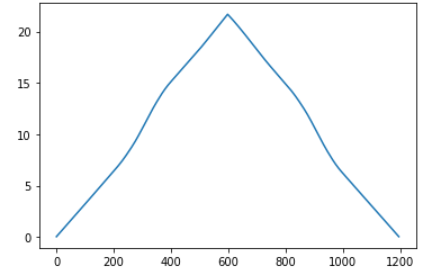
\includegraphics[scale=0.8]{images/task3_1.PNG} \\
\Tiny{Comparison of two signals with cross correlation}
\end{center}
The peak that can be seen in this plot represents the shift where the signals match the most. The x axis of this plot is twice the length of the signal and the highest point is right in the middle. This means that the signals doesn't need to be shifted at all. But this result is not correct because if we don't shift the signals, there is still a big error between them as we can see in the next plot with signal 0 and signal 1 from the assignment.\\


\begin{center}
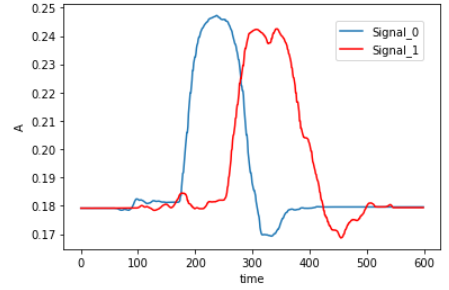
\includegraphics[scale=1.0]{images/task2_2.PNG} \\
\Tiny{Signal 0 and Signal 1 after cross correlation}
\end{center}

This error occurs because the cross correlation method only works if the direct current of the signals is 0. Therefore we calculated the mean of the signals and subtracted it from the signals.
In the next plot you can see the results obtained from this method with all signals of task 2. The subtraction of the mean was applied to all of the signals here. Now we can see that the signals are aligned better to each other. \\

\begin{center}
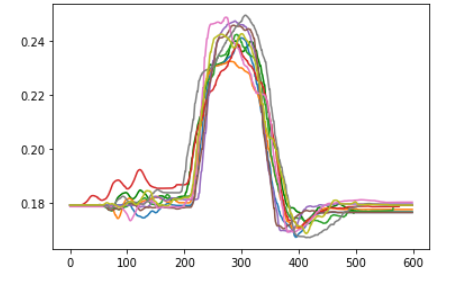
\includegraphics{images/task2_3.PNG} \\
\Tiny{All signals after cross correlation}
\end{center}



\section{Task 3}\label{section:task3}
\subsection{Introduction}
\label{sec:intro}
% Describe briefly how the method used in this task works.
Dynamic Time Warping (DTW) is a method which uses a cost matrix which describes the cost of all sample point pairs. Using this cost matrix we can compute the best pairs by selecting the path in the cost matrix with the lowest cumulative cost. This path gives rise to a similarity metric by calculating the average of the pairs of the path and a method to build two new signals which are the aligned versions of the input signals.

\subsection{Methods}
% Describe the problems you have found in this method, 
%Was this method solving the problem? in case not, why not? did you have to implement something else to make it work? describe your solutions and their limitations.

DTW is applied to two signals. When we then fit the signals together we compute two new signals. This means that these two signals have a different length than the input signals. This makes comparing more than two signals quite hard since all signals may have different lengths.

\subsection{Discussion}
%Describe briefly the results obtained after implementing this method. Analyze the results and include some metrics and plots that respect the error between the reference signal and the new aligned ones. We will discuss in class these results

When we compute the DTW distances between signal 0 and signals 1 to 9 we get the following:

\begin{align*}
    DTW_{distance}(0,1) &= 0.24670912010411336 \\
    DTW_{distance}(0,2) &= 0.34309190877520285 \\
    DTW_{distance}(0,3) &= 0.1528668532218145 \\
    DTW_{distance}(0,4) &= 0.2935484200879948  \\
    DTW_{distance}(0,5) &= 0.36787581848093565 \\
    DTW_{distance}(0,6) &= 0.3205108485271021 \\
    DTW_{distance}(0,7) &= 0.5018756539139264 \\
    DTW_{distance}(0,8) &= 0.38325670208522983 \\
    DTW_{distance}(0,9) &= 0.223140669858077 \\
\end{align*}
    
Interpreting these distances is quite hard since DTW does not give us some distance in a concrete interval (i.e.~a value between 0 and 1) but some value that is dependent on the length of the signals, the length of the resulting signals and the similarity between the signals. Something that $DTW_{distance}$ allows us to say is for example that signal 0 and signal 3 are more similar than signal 0 and signal 7. So, $DTW_{distance}$ allows us to compare two or more signals based on some common reference.

\begin{center}
    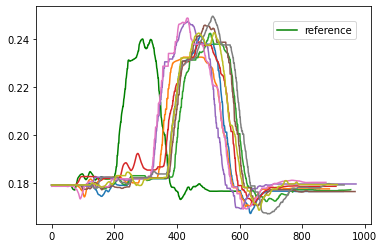
\includegraphics[scale=0.7]{images/dtw_aligned.png}\\
    \Tiny{Signals aligned with reference signal}
\end{center}

When aligning signals, DTW does not perform a simple shift but returns two new aligned signals. This is why the aligned signals in the above figure are not aligned to another at all. When using DTW the "correct" way we can only align two signals. 

\section{General Results}
% present some measures that compare the performance of both methods

Both methods have different properties which make them useful for different domains. When we look at the similarity measures given by cross correlation and dynamic time warping we get very different values. This is due to the way both methods work: cross correlation gives us a value describing the similarity; DTW gives us a value describing the cost of fitting the two signals. Those values are not directly comparable.

The results of fitting the signals with cross correlation are clearly better than with DTW. DTW does perform very differently than cross correlation and does not perform well when used in the way we did. On the other hand, when we plotted the two resulting signals of $DTW_{alignment}$ it was often difficult to distinguish between them. 

Additionally, we may emphasise that we observe a change in the time dimension when using DTW (in contrast to cross correlation). This property of DTW is very important when we want to use it in some system as it may impact the performance or even make it unsuitable. 

\section{General Discussion}
%Describe the main difference between the two methods used to align signals and their limitations. When one is better than the other one?

In this section we will discuss the qualities of the two methods. The first thing we noticed was that the Dynamic Time Warping method is more time consuming than the Cross-Correlation method with our implementation. This might be due to the construction of the matrix. An advantage of Dynamic Time Warping is that it can also be used when there are multiple different stretches within the signals, for example when there are two audio signals with speech where some parts are spoken slower and others faster. If we compare the alignment of the 9 signals with the reference signal we can see that with the cross correlation method all signals fit well with each other and also with the reference signal. With Dynamic Time Warping each signal fits well for the adjusted reference signal but not necessarily for the other signals and the original reference signal.This is because the lengths of both the reference signal and the signal to be aligned get adjusted differently for each signal. So for signals with a constant shift between each other the cross correlation method is suitable. It could also be used to search in a longer signal for a certain shorter feature. If each value of a signal corresponds to one or more values of the other signal like when you have to audio signals where the same text is spoken then you should use Dynamic Time Warping.

\section{Conclusion}
%Write a 5-10 line paragraph describing the main take-away

When comparing cross correlation and DTW we see that both methods address the same problem. However, they have different properties which make them suitable for different problem instances.
When we want to account for absolute shifts  and/or must not change the relative distances we have to use cross correlation. When we may change relative distances in signals we use DTW, as it can account for similar features which are differently shifted. 


\end{document}





